
% This is a simple template for a LaTeX document using the "article" class.
% See "book", "report", "letter" for other types of document.

\documentclass[10pt]{article} % use larger type; default would be 10pt

\usepackage[T1]{fontenc}
\usepackage[french]{babel}
\usepackage[utf8]{inputenc} % set input encoding (not needed with XeLaTeX)
% \usepackage{kpfonts}

%%% Examples of Article customizations
% These packages are optional, depending whether you want the features they provide.
% See the LaTeX Companion or other references for full information.

%%% PAGE DIMENSIONS
\usepackage{geometry} % to change the page dimensions
\geometry{a4paper} % or letterpaper (US) or a5paper or....
% THE MARGINS FOR DSA is 1.5cm
% \geometry{margin=1.5cm} % for example, change the margins to 2 inches all round
\geometry{margin=1cm} % for example, change the margins to 2 inches all round
\geometry{right = 1cm}
% \geometry{landscape} % set up the page for landscape
%   read geometry.pdf for detailed page layout information


% \usepackage[parfill]{parskip} % Activate to begin paragraphs with an empty line rather than an indent

%%% PACKAGES
\usepackage{booktabs} % for much better looking tables
\usepackage{array} % for better arrays (eg matrices) in maths
\usepackage{paralist} % very flexible & customisable lists (eg. enumerate/itemize, etc.)
\usepackage{verbatim} % adds environment for commenting out blocks of text & for better verbatim
% \usepackage{subfig} % make it possible to include more than one captioned figure/table in a single float
% These packages are all incorporated in the memoir class to one degree or another...

%%% HEADERS & FOOTERS
\usepackage{fancyhdr} % This should be set AFTER setting up the page geometry
% \pagestyle{fancy} % options: empty , plain , fancy

\usepackage{graphicx} % support the \includegraphics command and options
\usepackage{subcaption}
\usepackage{caption}
% \usepackage{tikz}

% \usepackage{uftsym}
\usepackage{dingbat} % For the pointy hands
\usepackage{pifont}
% \usepackage{xcolor} % For pretty colors
\usepackage[table]{xcolor}
\usepackage{tikz} % for nice pictures
\usepackage{blindtext}
\usepackage{wrapfig}
\usepackage{gensymb}
% \usepackage{table}

% COLORs
\definecolor{mygold}{RGB}{182, 153, 45}
\definecolor{mygreen}{RGB}{62, 171, 0}
\definecolor{dullgreen}{RGB}{165, 181, 45}
\definecolor{mypurp}{RGB}{84, 45, 181}
\definecolor{lpurp}{RGB}{146, 45, 203}
\definecolor{lgreen}{RGB}{143, 209, 68}


% \renewcommand{\headrule}{\color{gray}}
\renewcommand{\headrule}{\hbox to\headwidth{%
  \color{gray}\leaders\hrule height \headrulewidth\hfill}}

\renewcommand{\footrulewidth}{1pt}
% \renewcommand{\footrule}{\hbox to\headwirth{
%     \color{gray}\leaders\hrule height \footrulewidth\hfill}}

\renewcommand{\footrule}{{\color{gray}\vskip-\footruleskip\vskip-\footrulewidth \hrule width\headwidth height\footrulewidth\vskip\footruleskip}}

\fancyhf{}
\rhead{\textcolor{gray}{Séance TP 1}}
\chead{\color{gray} Travaux Pratiques}
% \lhead{Optimisation du GCC}
\lfoot{\color{gray}\textcopyright 2022 Evan Voyles}
\rfoot{\color{gray} Page \thepage\ sur 3}
\cfoot{\color{gray}Spécialité MAIN-3}
\footskip = 0pt
% \voffset = 10pt
% \headsep = 0pt
% \cfoot{\thepage\ of \pageref{LastPage}}

% \renewcommand{\headrulewidth}{0pt} % customise the layout...
% \lhead{}\chead{}\rhead{}
% \lfoot{}\cfoot{\thepage}\rfoot{}


\usepackage[absolute,overlay]{textpos} % Add text in any arbitrary position

%%% SECTION TITLE APPEARANCE
\usepackage{sectsty}
\allsectionsfont{\sffamily\mdseries\upshape} % (See the fntguide.pdf for font help)
% (This matches ConTeXt defaults)

%%% ToC (table of contents) APPEARANCE
\usepackage[nottoc,notlof,notlot]{tocbibind} % Put the bibliography in the ToC
\usepackage[titles,subfigure]{tocloft} % Alter the style of the Table of Contents
\renewcommand{\cftsecfont}{\rmfamily\mdseries\upshape}
\renewcommand{\cftsecpagefont}{\rmfamily\mdseries\upshape} % No bold!

%%% END Article customizations

%%% The "real" document content comes below...

\newcommand{\asgold}[1]{\textcolor{mygold}{{\bf#1}}}
\newcommand{\asgrey}[1]{\textcolor{gray}{{\bf#1}}}
\newcommand{\asred}[1]{\textcolor{red}{{\bf#1}}}
\newcommand{\asor}[1]{\textcolor{orange}{{\bf#1}}}
\newcommand{\ascy}[1]{\textcolor{cyan}{{\bf#1}}}
\newcommand{\asgr}[1]{\textcolor{mygreen}{{\bf#1}}}
\newcommand{\aspurp}[1]{\textcolor{mypurp}{{\bf#1}}}
\newcommand{\aslprp}[1]{\textcolor{lpurp}{{\bf#1}}}
\newcommand{\aslgrn}[1]{\textcolor{lgreen}{{\bf#1}}}


\begin{document}

% Template to make the document pretty
% This document was prepared to replicate the style of the Algorithmique
% Generale TP structure.

% \vspace{-10pt}
% This is the PERFECT SCALING, now we need to adjust the scale a little bit.
\begin{tikzpicture}[remember picture,overlay,yshift=-1.2cm, xshift=1.75cm] % LMAOOOOOO This is the EXACT POSITION!!!!
    \node at (0,0) {
\includegraphics[width=4.0cm,height=1.6cm]{media/1280px-Logo_Polytech_Sorbonne.png}};
\end{tikzpicture}

% \hspace{-5cm}
% \hspace{-1cm}
% \hspace{-1cm}

% \vspace{-1cm}
\vspace{0.3cm}

% {\raggedleft \color{mygold} Programmation en Python\\
% MAIN-3, année 2022\\
% Séance TP N\degree 1\\
% Février 2022\\
% VOYLES Evan\\}

{\raggedleft Printemps 2022\\
RAKOTOVAO Jonathan\\
VOYLES Evan\\}

% This vspace accomodates my name
\vspace{-0.42cm}
\vspace{1.23cm}

{\centering \Large \textbf{Circuits logiques}\par}
\vspace{0.4cm}
{\centering \large \textbf{TP 1}\par}

\noindent\rule{\textwidth}{1pt}


% {\Large \noindent \color{mygold} Objectif}

% {\color{mygold}\noindent\rule{\textwidth}{1pt}}
% \vspace{0cm}
% \begin{itemize}
%     \item[{\color{mygold}\ding{43}}] Expressions régulières.
% \end{itemize}

% \vspace{1.2cm}
% {\color{dullgreen}\noindent \Large \bf Problème}

% \vspace{-0.28cm}
% {\vspace{0cm}\color{dullgreen}\noindent\rule{\textwidth}{1pt}}

% \begin{textblock*}{10cm}(13.58cm,7.2cm) % {block width} (coords)
%     \Large \aspurp{[Expression régulières]}
% \end{textblock*}


% \section*{\aslprp{Enseignements première année (L3)}}
% \input{premiere_annee.tex}
% \section*{\aslprp{Enseignements deuxième année (L4)}}
% \input{deuxieme_annee.tex}

\vspace{0.7cm}
{\noindent \Large \bf Objectifs}
\begin{itemize}
    \item [\ding{78}] Se familiariser avec logisim
    \item [\ding{78}] Modéliser une formule logique
    \item [\ding{78}] Simuler un circuit logique
\end{itemize}
% \noindent\rule{\textwidth}{1pt}


\section{Combinatorial Circuit}

% \hspace{1cm}
\begin{table}[h!]
    \hspace{2cm}
    \begin{minipage}{0.5\linewidth}
        \begin{tabular}{l | l |l | c |l}
            $a$ & $b$ & $c$ & ($b \cdot \bar c$) & s \\
            \hline
            0 & 0 & 0 & 0                                              & 0 \\
            0 & 0 & 1 & 0                                              & 0 \\
            0 & 1 & 0 & 1                                              & 1 \\
            0 & 1 & 1 & 0                                              & 0 \\
            1 & 0 & 0 & 0                                              & 1 \\
            1 & 0 & 1 & 0                                              & 1 \\
            1 & 1 & 0 & 1                                              & 1 \\
            1 & 1 & 1 & 0                                              & 1
        \end{tabular}
    \end{minipage}

    % \begin{minipage}{0.5\linewidth}
        % \includegraphics{}
    % \end{minipage}


\end{table}

\section{Circuit 7 segments}
\begin{itemize}
    \item [\ding{78}] Ecrire le table de vérité du sous-circuit \texttt{Bit1}
\end{itemize}

Le \texttt{Bit1} doit être allumé pour les chiffres (en décimal) qui appartient à l'ensemble $\{0, 1, 3, 4, 5, 6, 7, 8, 9\}$. Sa table de
vérité est donc:

\begin{table}[h!]
    \hspace{2cm}
    \begin{tabular}{l|llll |l}
    Chiffre & $a$ & $b$ & $c$ & $d$ & $s$ \\
    \hline
    0       & 0 & 0 & 0 & 0 & 1 \\
    1       & 0 & 0 & 0 & 1 & 1 \\
    2       & 0 & 0 & 1 & 0 & 0 \\
    3       & 0 & 0 & 1 & 1 & 1 \\
    4       & 0 & 1 & 0 & 0 & 1 \\
    5       & 0 & 1 & 0 & 1 & 1 \\
    6       & 0 & 1 & 1 & 0 & 1 \\
    7       & 0 & 1 & 1 & 1 & 1 \\
    8       & 1 & 0 & 0 & 0 & 1 \\
    9       & 1 & 0 & 0 & 1 & 1 \\
    E       & 1 & x & x & x & 0
    \end{tabular}
    \end{table}

% \newpage

Pour construire le sous-circuit \texttt{Bit4}, on procède d'une manière analogue du \texttt{Bit4}. On doit tout d'abord établir
pour quel chiffres doit-on allumer la position $b4$ dans le circuit 7 segments. Une analyse nous révèle que \texttt{Bit4} doit être allumé
pour les chiffres $\{0, 4, 5, 6, 8, 9\}$.

\newpage

\begin{table}[h!]
    \hspace{2cm}
    \begin{tabular}{l|llll|l}
    Chiffre & $a$ & $b$ & $c$ & $d$ & $s$ \\
    \hline
    0       & 0 & 0 & 0 & 0 & 1 \\
    1       & 0 & 0 & 0 & 1 & 0 \\
    2       & 0 & 0 & 1 & 0 & 0 \\
    3       & 0 & 0 & 1 & 1 & 0 \\
    4       & 0 & 1 & 0 & 0 & 1 \\
    5       & 0 & 1 & 0 & 1 & 1 \\
    6       & 0 & 1 & 1 & 0 & 1 \\
    7       & 0 & 1 & 1 & 1 & 0 \\
    8       & 1 & 0 & 0 & 0 & 1 \\
    9       & 1 & 0 & 0 & 1 & 1 \\
    E       & 1 & x & x & x & 1
    \end{tabular}
    \end{table}

    A partir de cette table de vérité on a pu générer automatiquement le circuit suivant

    \begin{figure}[h!]
        \centering
        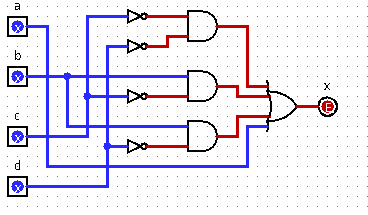
\includegraphics[width=0.4\textwidth]{media/bit4.png}
        \caption{Circuit de \texttt{Bit4}. Il est encodé par la fonction booléenne $s = a + b\bar d + b\bar c + \bar c \bar d$}
    \end{figure}

    Le bug qu'on a trouvé c'est que \texttt{Bit6} est allumé incorrectement quand on veut visualiser le chiffre 7. Alors pour résoudre le problème
    on modifie la table de vérité de \texttt{Bit6} pour que $\texttt{Bit6}(0,1,1,1) = 0$. Enfin on génère le circuit selon la table modifié et on
    trouve que le bug est résolu.

\section{Conception d'une unité arithmétique et logique (ALU)}

    L'opération d'addition en binaire est presque pareil de celui en décimal, pourtant en binaire on a que $2$ chiffres, $\{0, 1\}$, pour représenter les nombres.
    De même, il s'agit d'additioner deux nombres chiffres par chiffres, en gardant un chiffre de retenue quand on dépasse le maximum chiffre qu'on a dans notre base.

    \begin{table}[h!]
        \hspace{1cm}
        \begin{tabular}{lll|l|l|l}
        $a$ & $b$ & $c$ & $O[0]$ & V & cout \\
        \hline
        0 & 0 & 0 & 0        & 0 & 0    \\
        0 & 0 & 1 & 1        & 0 & 0    \\
        0 & 1 & 0 & 1        & 0 & 0    \\
        0 & 1 & 1 & 0        & 1 & 1    \\
        1 & 0 & 0 & 1        & 0 & 0    \\
        1 & 0 & 1 & 0        & 1 & 1    \\
        1 & 1 & 0 & 0        & 1 & 1    \\
        1 & 1 & 1 & 1        & 1 & 1
        \end{tabular}
        \end{table}

% \pagestyle{fancy}
Pour transformer un nombre en sa version négative selon l'encodage de complément à 2, on prend le complément à 1 - c'est-à-dire l'inversion de tous les bits d'un nombre - et
après on ajoute 1 à ce nombre inversé. Si on dédie un bit d'entré pour choisir l'opération à executer (1 pour la soustraction, 0 pour l'addition), on peut utiliser une porte
XOR avec le bit d'opération et chaque bit de notre entier de 32bits pour inverser les bits quand le bit d'opération est allumé. Pour visualiser cela on écrit la table de vérité
d'une XOR.

\begin{table}[h!]
    \hspace{1cm}
    \begin{tabular}{ll|l}
    $a$ & $b$ & $c$ \\
    \hline
    0 & 0 & 0 \\
    0 & 1 & 1 \\
    1 & 0 & 1 \\
    1 & 1 & 0
    \end{tabular}
    \end{table}

    Si on concentre sur le moitié en bas où $a$ est vrai, on remarque que la value de $c$ est tout simplement $\bar b$. Alors on donne a manger
    tout les 32 bits dans 32 portes XOR pour avoir le complément à 1 du nombre et ensuite on donne en entré ce nombre plus 1 pour faire une addition, où le `plus 1'
    remplit le vide du bit de retenue en entré du 32-bit adder. Le circuit est bouclé, on a con\c cu une ALU.

\end{document}
